
\begin{figure}[!htbp]
    \centering
    \begin{subfigure}[b]{0.5\textwidth}
      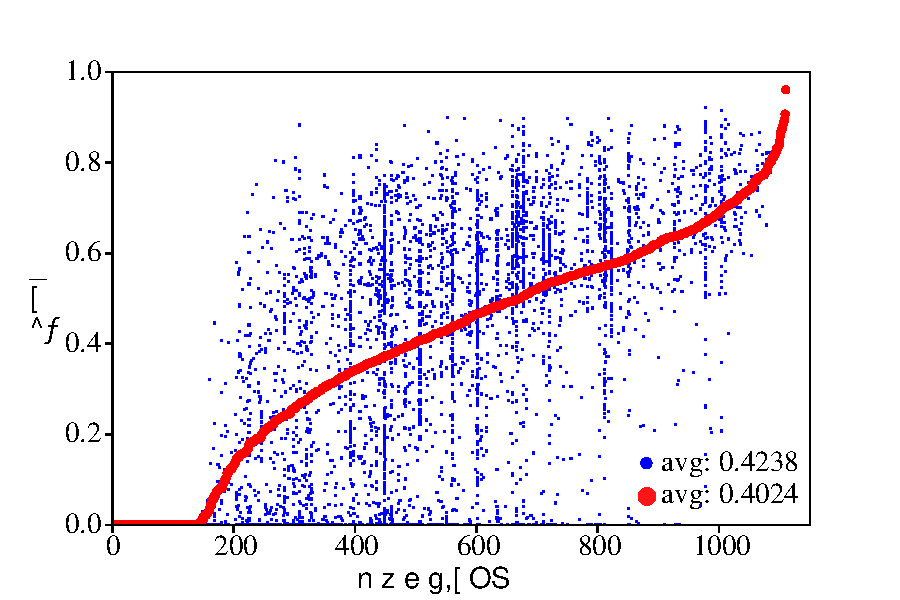
\includegraphics[width=\textwidth]{Img/fig_4_fidelity_base.pdf}
      \caption{Transformer}
      \label{fig:4_fidelity_base}
    \end{subfigure}%
    ~% add desired spacing
    \begin{subfigure}[b]{0.5\textwidth}
      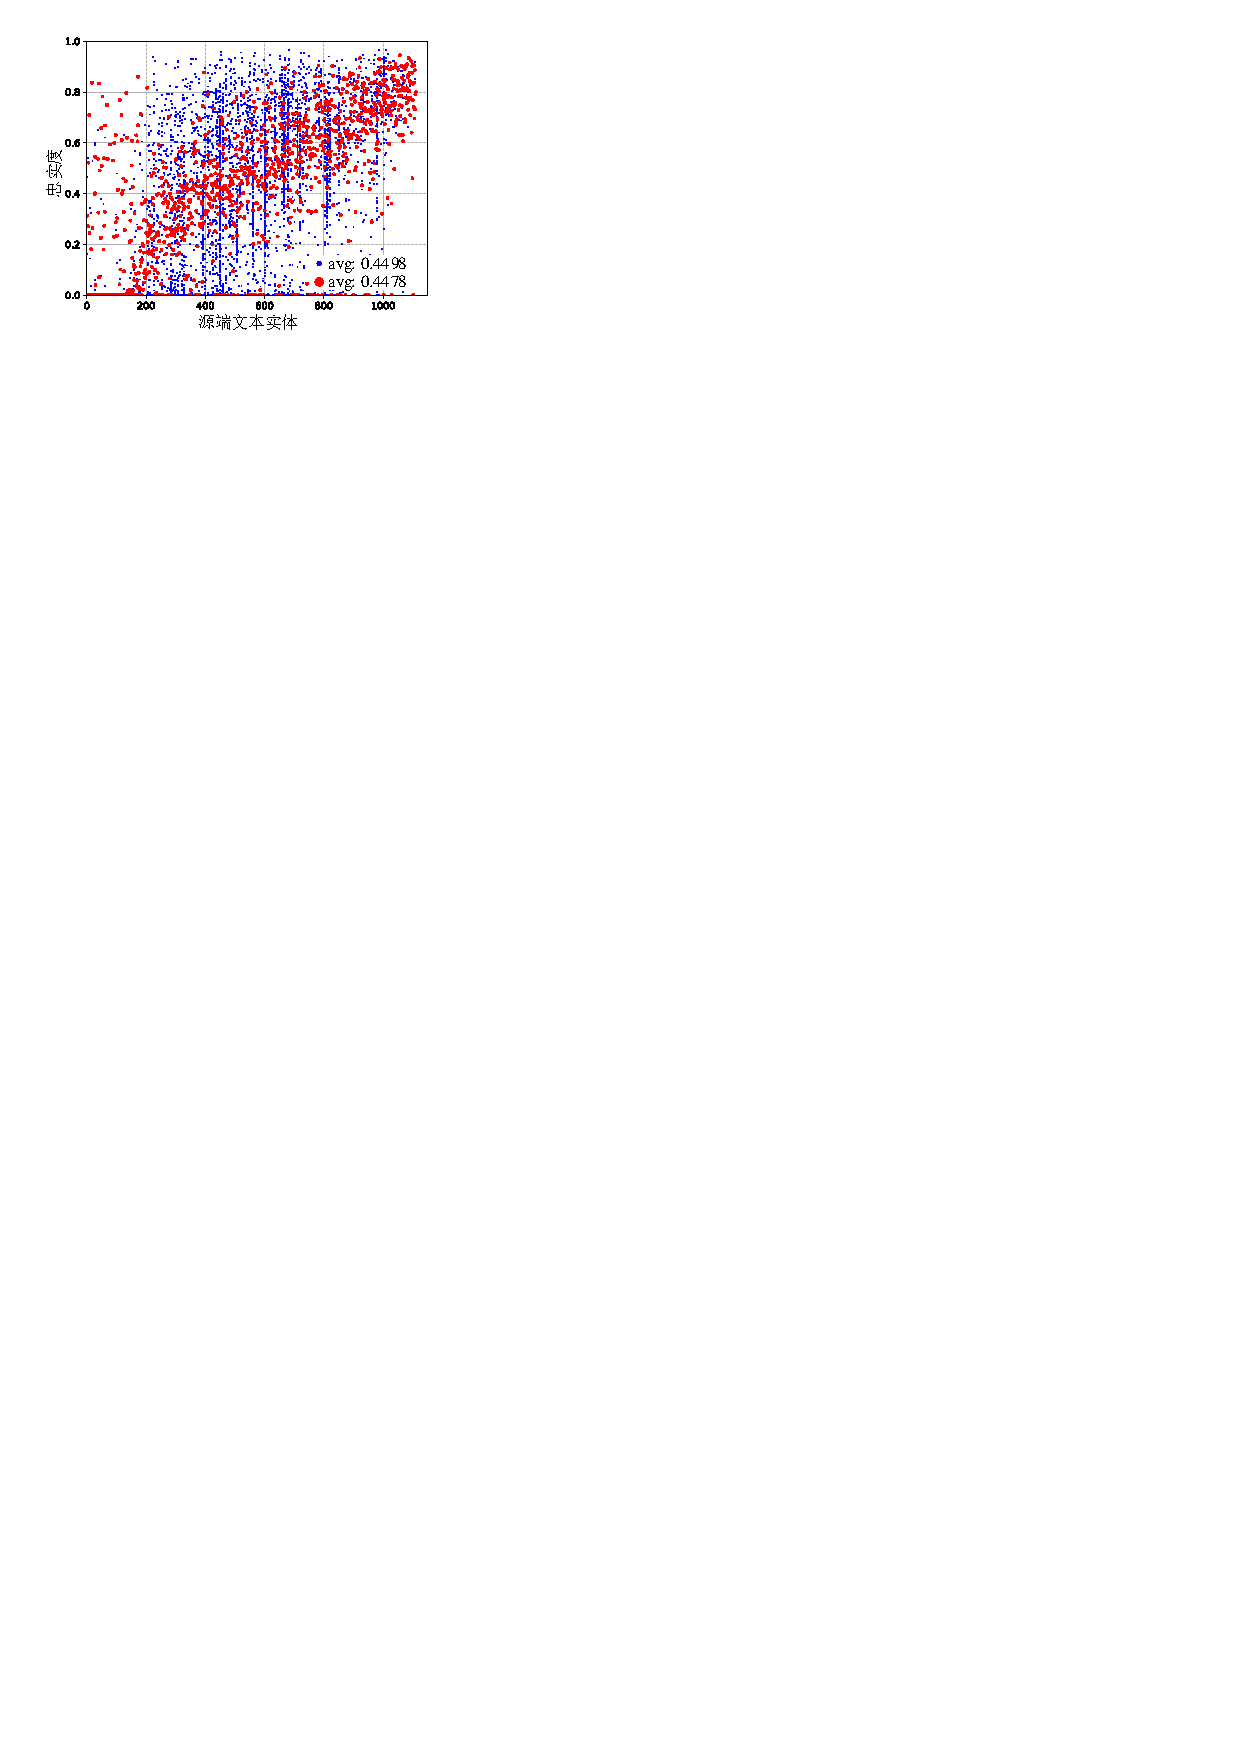
\includegraphics[width=\textwidth]{Img/fig_4_fidelity_cer_baseorder.pdf}
      \caption{CER-NMT}
      \label{fig:4_fidelity_cer_baseorder}
    \end{subfigure}
    \\% line break
    \begin{subfigure}[b]{0.5\textwidth}
      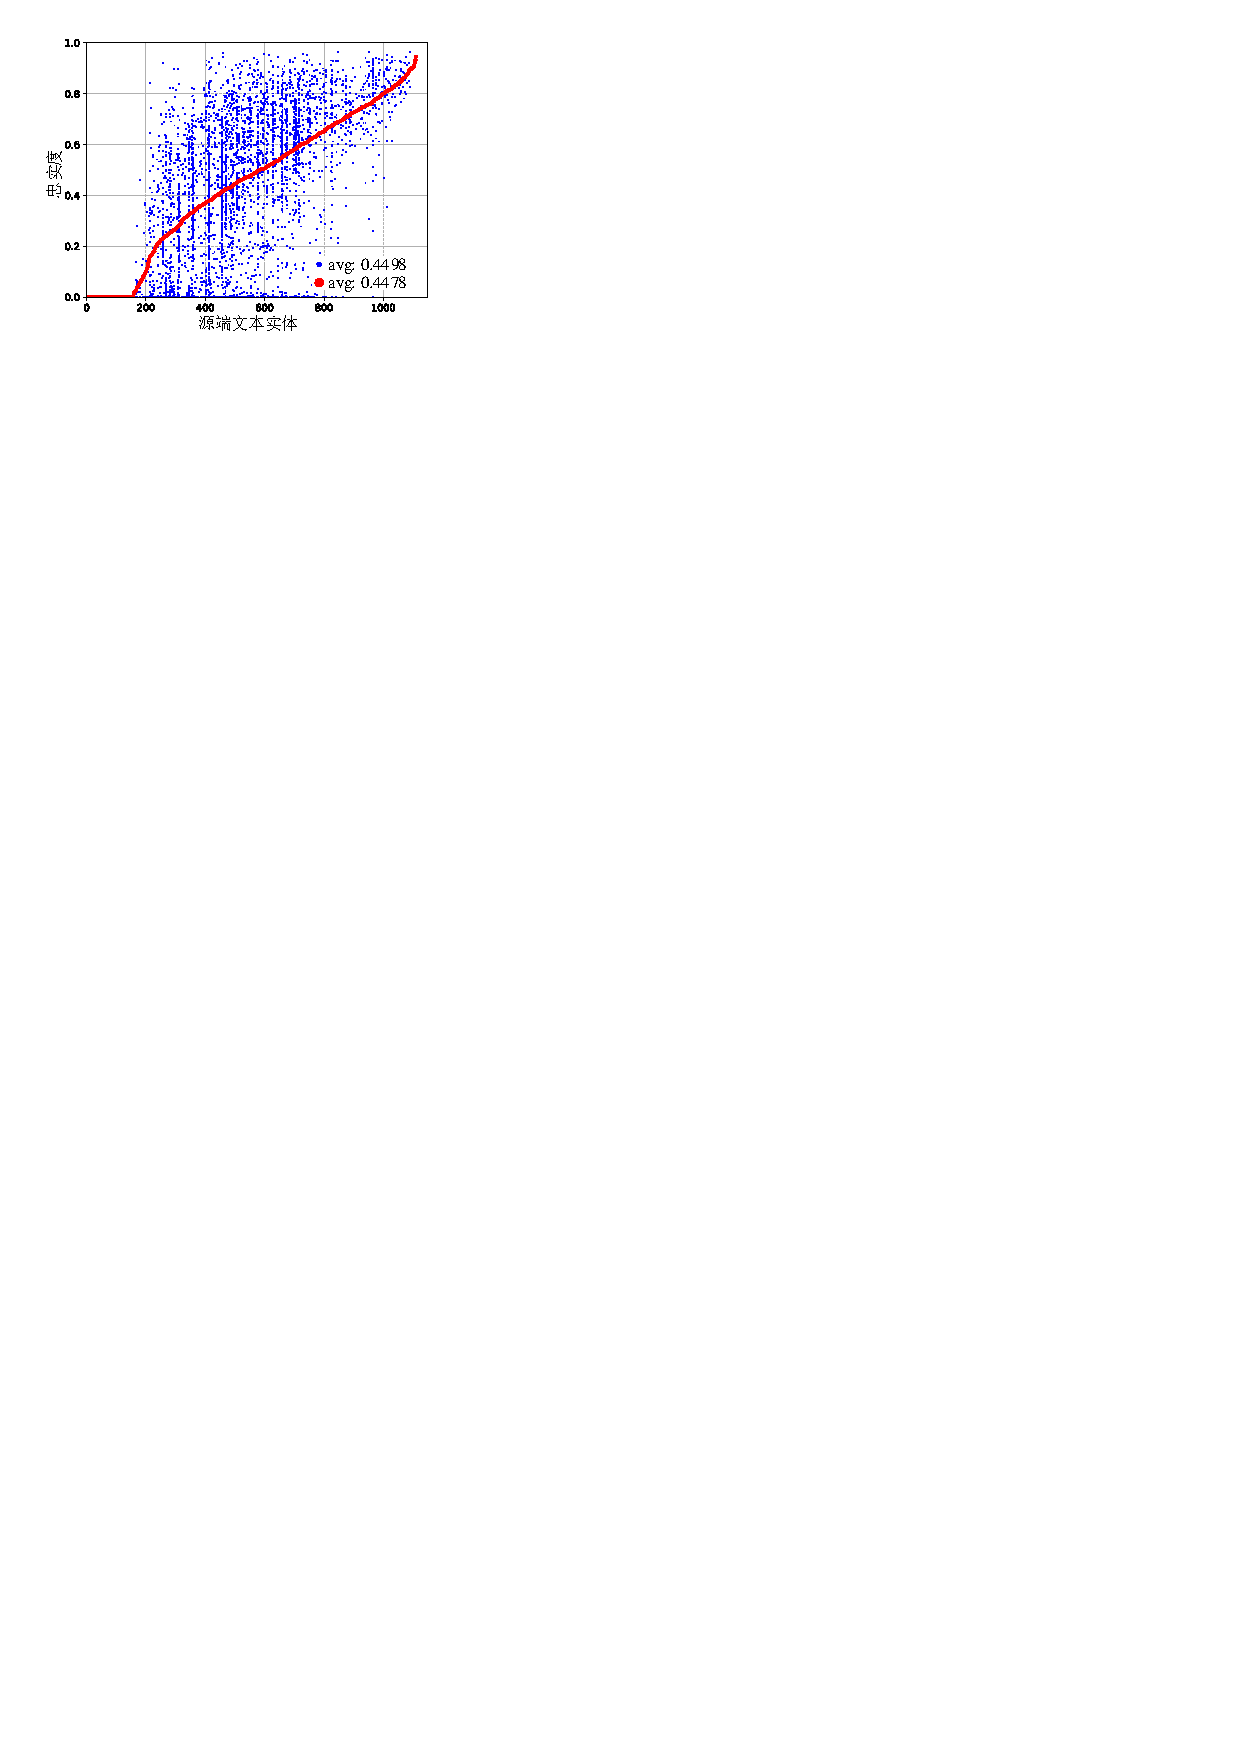
\includegraphics[width=\textwidth]{Img/fig_4_fidelity_cer_selforder.pdf}
      \caption{实体重排序的CER-NMT}
      \label{fig:4_fidelity_cer_selforder}
    \end{subfigure}%
    ~% add desired spacing
    \begin{subfigure}[b]{0.5\textwidth}
      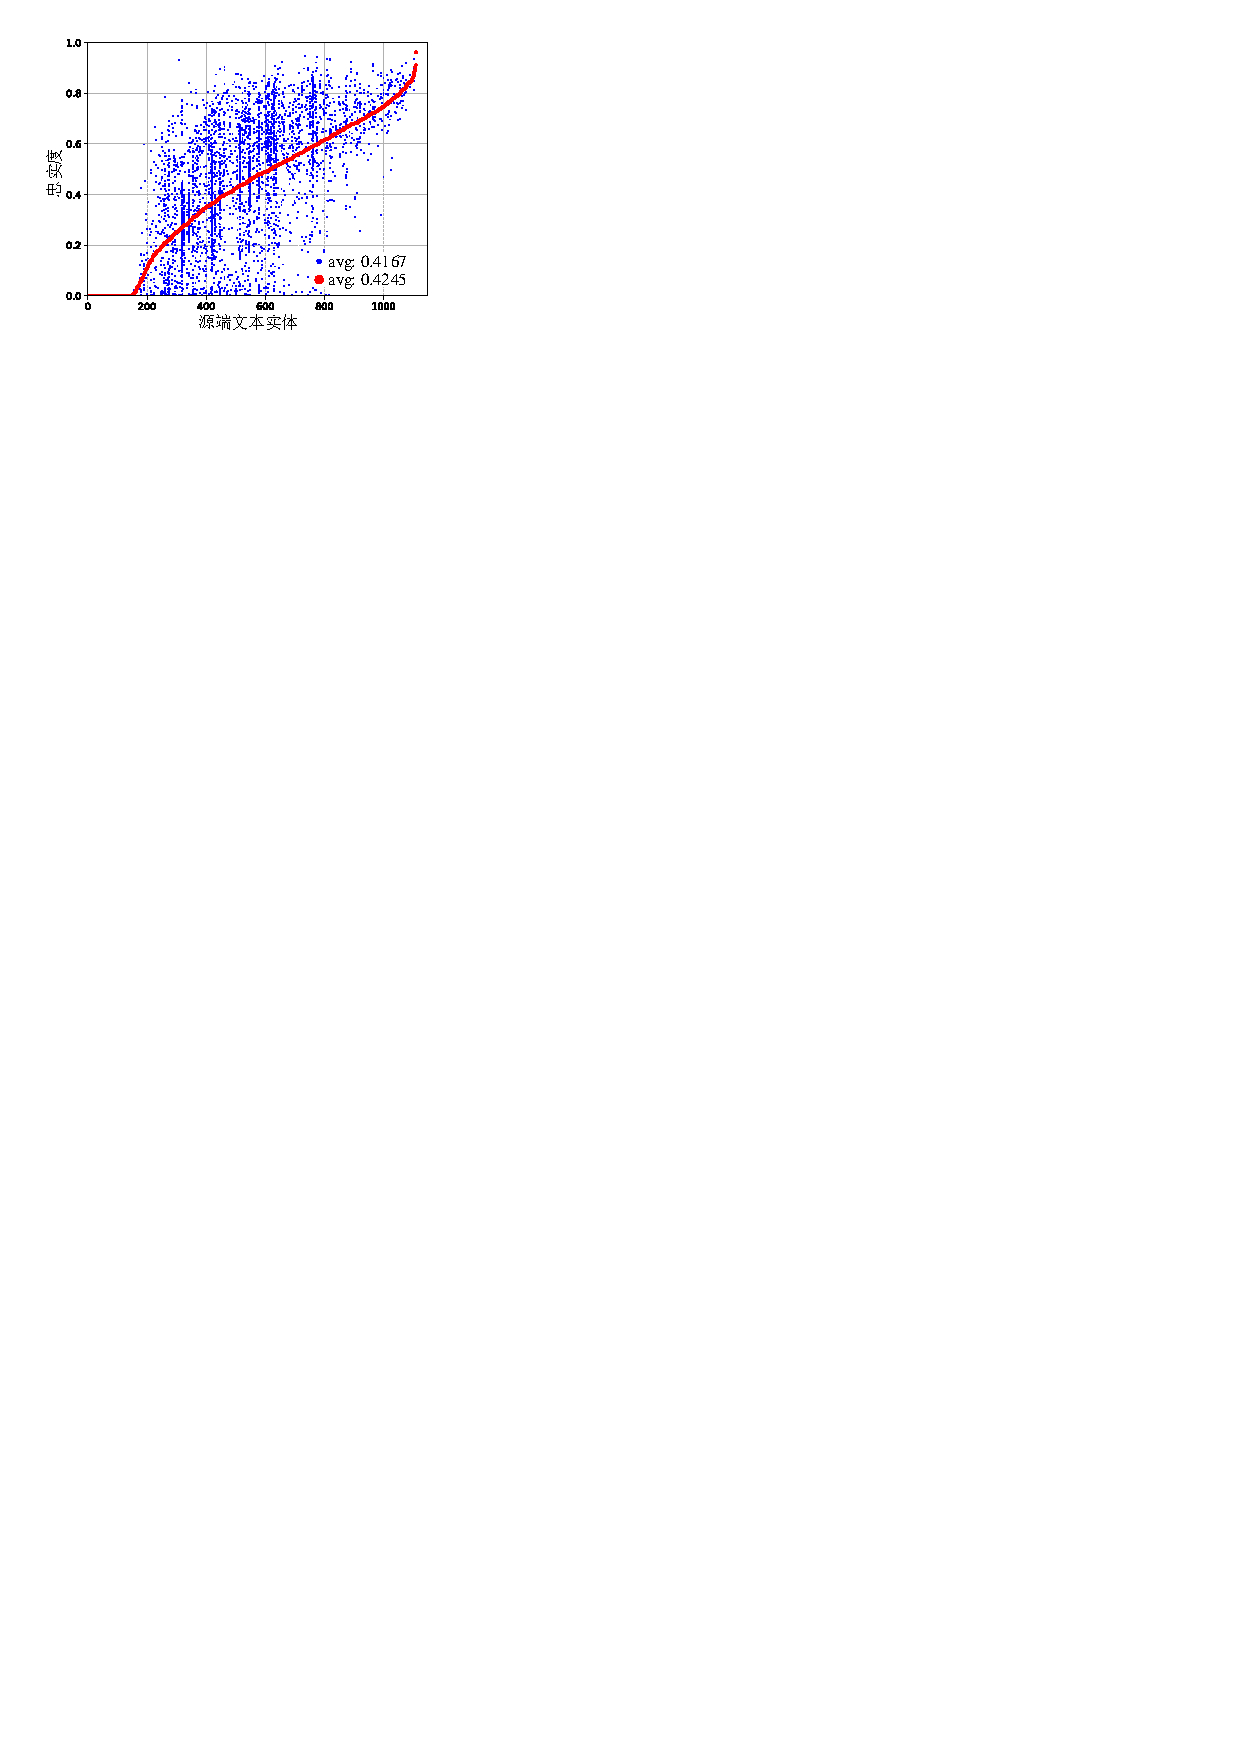
\includegraphics[width=\textwidth]{Img/fig_4_fidelity_tner.pdf}
      \caption{TNER-NMT}
      \label{fig:4_fidelity_tner}
    \end{subfigure}
    \bicaption{文本实体在不同模型下的忠实度}{The fidelity of textual entities on different models}
    \label{fig:4_fidelity}
\end{figure}